% Uebung 39) dynamisches Mikrofon nach Brinkmeyer
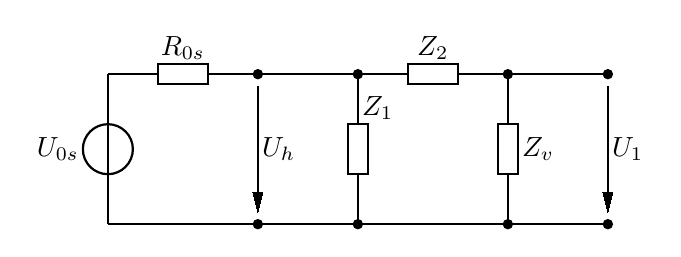
\begin{tikzpicture}[scale=2.54]%
% dpic version 2024.01.01 option -g for TikZ and PGF 1.01
\ifx\dpiclw\undefined\newdimen\dpiclw\fi
\global\def\dpicdraw{\draw[line width=\dpiclw]}
\global\def\dpicstop{;}
\dpiclw=0.8bp
\dpiclw=0.8bp
\dpicdraw (0,0)
 --(0,-0.25)\dpicstop
\dpicdraw (0,-0.375) circle (0.049213in)\dpicstop
\dpicdraw (0,-0.25)
 --(0,-0.5)\dpicstop
\dpicdraw (0,-0.5)
 --(0,-0.75)\dpicstop
\draw (-0.125,-0.375) node[left=-2bp]{$ U_{0s}$};
\dpicdraw (0,0)
 --(0.25,0)\dpicstop
\dpicdraw (0.5,0)
 --(0.5,0.05)
 --(0.25,0.05)
 --(0.25,-0.05)
 --(0.5,-0.05)
 --(0.5,0)\dpicstop
\dpicdraw (0.5,0)
 --(0.75,0)\dpicstop
\draw (0.375,0.05) node[above=-2bp]{$ R_{0s}$};
\dpicdraw[fill=black](0.75,0) circle (0.007874in)\dpicstop
\dpicdraw[fill=black](0.75,-0.75) circle (0.007874in)\dpicstop
\filldraw[line width=0bp](0.725,-0.59)
 --(0.75,-0.69)
 --(0.775,-0.59) --cycle\dpicstop
\dpicdraw (0.75,-0.06)
 --(0.75,-0.667094)\dpicstop
\draw (0.75,-0.375) node[right=-2bp]{$ U_h$};
\dpicdraw (0.75,0)
 --(1.25,0)\dpicstop
\dpicdraw[fill=black](1.25,0) circle (0.007874in)\dpicstop
\dpicdraw (1.25,0)
 --(1.25,-0.25)\dpicstop
\dpicdraw (1.25,-0.5)
 --(1.3,-0.5)
 --(1.3,-0.25)
 --(1.2,-0.25)
 --(1.2,-0.5)
 --(1.25,-0.5)\dpicstop
\dpicdraw (1.25,-0.5)
 --(1.25,-0.75)\dpicstop
\draw (1.25,-0.25) node[above right=-2bp]{$ Z_1$};
\dpicdraw[fill=black](1.25,-0.75) circle (0.007874in)\dpicstop
\dpicdraw (1.25,0)
 --(1.5,0)\dpicstop
\dpicdraw (1.75,0)
 --(1.75,0.05)
 --(1.5,0.05)
 --(1.5,-0.05)
 --(1.75,-0.05)
 --(1.75,0)\dpicstop
\dpicdraw (1.75,0)
 --(2,0)\dpicstop
\draw (1.625,0.05) node[above=-2bp]{$ Z_2$};
\dpicdraw[fill=black](2,0) circle (0.007874in)\dpicstop
\dpicdraw (2,0)
 --(2,-0.25)\dpicstop
\dpicdraw (2,-0.5)
 --(2.05,-0.5)
 --(2.05,-0.25)
 --(1.95,-0.25)
 --(1.95,-0.5)
 --(2,-0.5)\dpicstop
\dpicdraw (2,-0.5)
 --(2,-0.75)\dpicstop
\draw (2.05,-0.375) node[right=-2bp]{$ Z_v$};
\dpicdraw[fill=black](2,-0.75) circle (0.007874in)\dpicstop
\dpicdraw (2,0)
 --(2.5,0)\dpicstop
\dpicdraw[fill=black](2.5,0) circle (0.007874in)\dpicstop
\dpicdraw[fill=black](2.5,-0.75) circle (0.007874in)\dpicstop
\filldraw[line width=0bp](2.475,-0.59)
 --(2.5,-0.69)
 --(2.525,-0.59) --cycle\dpicstop
\dpicdraw (2.5,-0.06)
 --(2.5,-0.667094)\dpicstop
\draw (2.5,-0.375) node[right=-2bp]{$ U_1$};
\dpicdraw (2.5,-0.75)
 --(0,-0.75)\dpicstop
\end{tikzpicture}%
